\documentclass{article}
\usepackage{geometry}
\usepackage{tikz,tkz-graph,graphicx}
\usepackage{xcolor}
\usetikzlibrary{arrows.meta,positioning,shapes}
\usepackage[utf8]{inputenc}
\usepackage{tikz, pgfplots}
\usepackage[T1]{fontenc}
\usepackage{adjustbox}
\usetikzlibrary{positioning, automata, calc}
\pgfplotsset{compat = 1.18}
\title{Practice Problems}
\author{Nilanjana}
\begin{document}
\maketitle
\tableofcontents
\clearpage


\section{}
\vspace{1cm}
\begin{center}
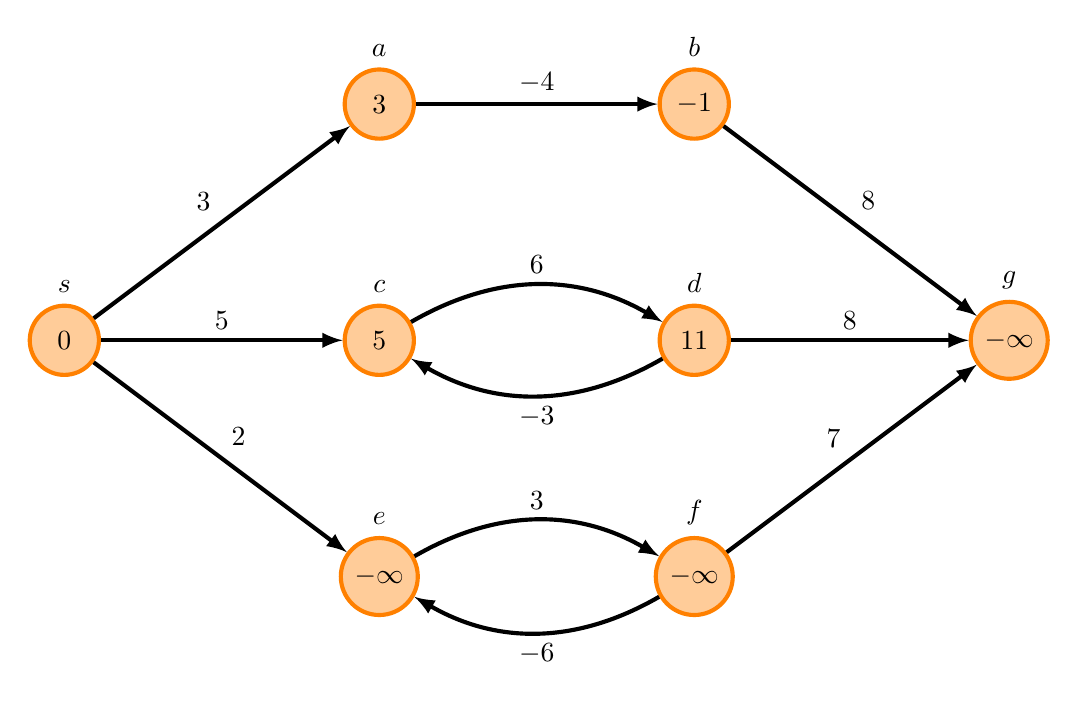
\begin{tikzpicture}[
    ->, >=latex, % Use LaTeX-style arrows
    line width=1.5pt, % Increase the thickness of the arrow lines
    >=latex, scale=2, % Scale the arrowheads
    node distance=4cm and 0.2cm, % Adjust node distance (horizontal and vertical)
    auto % Automatically position labels
]

% Nodes with labels
\node[state,fill=orange!40,draw=orange ,label=above:{$s$}] (A) {$0$};
\node[state,fill=orange!40,draw=orange , label=above:{$c$}] (B) [right of=A] {$5$};
\node[state,fill=orange!40,draw=orange , label=above:{$d$}] (C) [right of=B] {$11$};
\node[state,fill=orange!40,draw=orange , label=above:{$g$}] (D) [right of=C] {$-\infty$};

\node[state,fill=orange!40,draw=orange , label=above:{$a$}] (E) [above of=B,yshift=-1cm] {$3$};
\node[state, fill=orange!40,draw=orange ,label=above:{$b$}] (F) [above of=C,yshift=-1cm] {$-1$};

\node[state,fill=orange!40,draw=orange , label=above:{$e$}] (G) [below of=B,yshift=1cm] {$-\infty$};
\node[state, fill=orange!40,draw=orange ,label=above:{$f$}] (H) [below of=C,yshift=1cm] {$-\infty$};

% Edges with labels
\path (A) edge node {$5$} (B);
\path (B) edge[bend left] node {$6$} (C);
\path (C) edge[bend left] node {$-3$} (B);
\path (C) edge node {$8$} (D);

\path (A) edge node {$3$} (E);
\path (E) edge node {$-4$} (F);
\path (F) edge node {$8$} (D);

\path (A) edge node {$2$} (G);
\path (G) edge[bend left] node {$3$} (H);
\path (H) edge[bend left] node {$-6$} (G);
\path (H) edge node {$7$} (D);

\end{tikzpicture}
\end{center}

\vspace{1cm}
\section{}
\vspace{1cm}
\begin{center}
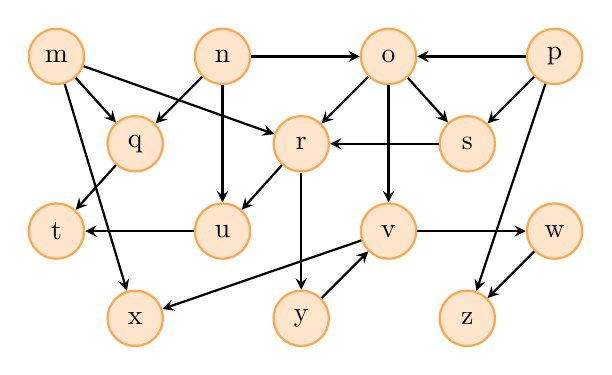
\begin{tikzpicture}[auto, node/.style = {circle, draw = orange!70, fill = orange!100!yellow!20, minimum size = 2em, node distance = 6em}, >=stealth, thick]
	\node[node](m){m};
	\node[node](n)[right of = m]{n};
	\node[node](o)[right of = n]{o};
	\node[node](p)[right of = o]{p};
	\node[node](q)[below of = m, xshift = 1cm, yshift = 1cm]{q};
	\node[node](r)[right of = q]{r};
	\node[node](s)[right of = r]{s};
	\node[node](t)[below of = q, xshift = -1cm, yshift = 1cm]{t};
	\node[node](u)[right of = t]{u};
	\node[node](v)[right of = u]{v};
	\node[node](w)[right of = v]{w};
	\node[node](x)[below of = t, xshift = 1cm, yshift = 1cm]{x};
	\node[node](y)[right of = x]{y};
	\node[node](z)[right of = y]{z};
	
	\path[->](n) edge (o);
	\path[->](p) edge (o);
	\path[->](n) edge (q);
	\path[->](m) edge (q);
	\path[->](m) edge (r);
	\path[->](s) edge (r);
	\path[->](q) edge (t);
	\path[->](u) edge (t);
	\path[->](v) edge (w);
	\path[->](m) edge (x);
	\path[->](v) edge (x);
	\path[->](p) edge (z);
	\path[->](w) edge (z);
	\path[->](r) edge (y);
	\path[->](y) edge (v);
	\path[->](p) edge (s);
	\path[->](r) edge (u);
	\path[->](n) edge (u);
	\path[->](o) edge (s);
	\path[->](o) edge (r);
	\path[->](o) edge (v);

\end{tikzpicture}
\end{center}

\vspace{1cm}
\section{}
\vspace{1cm}
\begin{adjustbox}{width = \textwidth}
\tikzstyle{line} = [draw, >=latex, rounded corners]
\begin{tikzpicture}[auto,
		alpha_node/.style = {circle, draw = white, inner sep = 0pt},
		nil_node/.style = {circle, draw = white, inner sep = 0pt, label = right:{$L.nil$}},
		blue_node/.style = {rectangle, draw, fill = blue!30!, minimum height = 2em, minimum width = 3em, inner sep = 0pt},
		orange_node/.style = {rectangle, draw, fill = orange!30!, minimum height = 2em, minimum width = 3em, inner sep = 0pt},
		scale = 5,
		->, >=latex, % Use LaTeX-style arrows
    		line width=1.5pt, % Increase the thickness of the arrow lines
    		>=latex, scale=2, % Scale the arrowheads
		]
	\node[alpha_node, label=left:{$(a)$}] (a) {};
	\node[alpha_node, label = left:{$(b)$}] (b) [below of = a, yshift = -1cm]{};
	\node[alpha_node, label = left:{$(c)$}] (c) [below of = b, yshift = -1cm]{};
	\node[alpha_node, label = left:{$(d)$}] (d) [below of = c, yshift = -1cm]{};
	\node[alpha_node, label = left:{$(e)$}] (e) [below of = d, yshift = -1cm]{};
	
	\node[nil_node] (1) [right of = a, xshift = 1cm]{};
	\node[nil_node] (2) [right of = b, xshift = 1cm]{};
	\node[nil_node] (3) [right of = c, xshift = 1cm]{};
	\node[nil_node] (4) [right of = d, xshift = 1cm]{};
	\node[nil_node] (5) [right of = e, xshift = 1cm]{};
	
	%row-1
	\node[blue_node] (r11) [right of = 1, xshift = 3cm]{};
	\node[blue_node] (r12) [right of = r11, xshift = 0cm]{};
	\node[blue_node] (r13) [right of = r12, xshift = 0cm]{};
	
	%row-2
	\node[blue_node] (r21) [right of = 2, xshift = 3cm]{};
	\node[blue_node] (r22) [right of = r21, xshift = 0cm]{};
	\node[blue_node] (r23) [right of = r22, xshift = 0cm]{};
	\node[orange_node] (o21) [right of = r21, xshift = 5cm]{};
	\node[orange_node] (o22) [right of = o21]{$9$};
	\node[orange_node] (o23) [right of = o22]{};
	\node[orange_node] (o31) [right of = o23, xshift = 3cm]{};
	\node[orange_node] (o32) [right of = o31]{$16$};
	\node[orange_node] (o33) [right of = o32]{};
	\node[orange_node] (o41) [right of = o33, xshift = 3cm]{};
	\node[orange_node] (o42) [right of = o41]{$4$};
	\node[orange_node] (o43) [right of = o42]{};
	\node[orange_node] (o51) [right of = o43, xshift = 3cm]{};
	\node[orange_node] (o52) [right of = o51]{$1$};
	\node[orange_node] (o53) [right of = o52]{};
	
	%row-3
	\node[blue_node] (r31) [right of = 3, xshift = 3cm]{};
	\node[blue_node] (r32) [right of = r31, xshift = 0cm]{};
	\node[blue_node] (r33) [right of = r32, xshift = 0cm]{};
	\node[orange_node] (f) [right of = r31, xshift = 5cm]{};
	\node[orange_node] (g) [right of = f]{$25$};
	\node[orange_node] (h) [right of = g]{};
	\node[orange_node] (i) [right of = h, xshift = 3cm]{};
	\node[orange_node] (j) [right of = i]{$9$};
	\node[orange_node] (l) [right of = j]{};
	\node[orange_node] (k) [right of = l, xshift = 3cm]{};	
	\node[orange_node] (m) [right of = k]{$16$};
	\node[orange_node] (n) [right of = m]{};
	\node[orange_node] (o) [right of = n, xshift = 3cm]{};
	\node[orange_node] (p) [right of = o]{$4$};
	\node[orange_node] (q) [right of = p]{};
	\node[orange_node] (r) [right of = q, xshift = 3cm]{};
	\node[orange_node] (s) [right of = r]{$1$};
	\node[orange_node] (t) [right of = s]{};
	
	%row-4
	\node[blue_node] (r41) [right of = 4, xshift = 3cm]{};
	\node[blue_node] (r42) [right of = r41, xshift = 0cm]{};
	\node[blue_node] (r43) [right of = r42, xshift = 0cm]{};
	\node[orange_node] (u) [right of = r43, xshift = 3cm]{};
	\node[orange_node] (v) [right of = u]{$25$};
	\node[orange_node] (w) [right of = v]{};
	\node[orange_node] (x) [right of = w, xshift = 3cm]{};
	\node[orange_node] (y) [right of = x]{$9$};
	\node[orange_node] (z) [right of = y]{};
	\node[orange_node] (uu) [right of = z, xshift = 3cm]{};	
	\node[orange_node] (vv) [right of = uu]{$16$};
	\node[orange_node] (ww) [right of = vv]{};
	\node[orange_node] (xx) [right of = ww, xshift = 3cm]{};
	\node[orange_node] (yy) [right of = xx, xshift = 0cm]{$4$};
	\node[orange_node] (zz) [right of = yy]{};
	
	%row-5
	\node[blue_node] (r51) [right of = 5, xshift = 3cm]{};
	\node[blue_node] (r52) [right of = r51, xshift = 0cm]{};
	\node[blue_node] (r53) [right of = r52, xshift = 0cm]{};
	\node[orange_node] (5a) [right of = r53, xshift = 3cm]{};
	\node[orange_node] (5b) [right of = 5a]{$25$};
	\node[orange_node] (5c) [right of = 5b]{};
	\node[orange_node] (5d) [right of = 5c, xshift = 3cm]{};
	\node[orange_node] (5e) [right of = 5d]{$9$};
	\node[orange_node] (5f) [right of = 5e]{};
	\node[orange_node] (5g) [right of = 5f, xshift = 3cm]{};	
	\node[orange_node] (5h) [right of = 5g]{$36$};
	\node[orange_node] (5i) [right of = 5h]{};
	\node[orange_node] (5j) [right of = 5i, xshift = 3cm]{};
	\node[orange_node] (5k) [right of = 5j]{$16$};
	\node[orange_node] (5l) [right of = 5k]{};
	\node[orange_node] (5m) [right of = 5l, xshift = 3cm]{};
	\node[orange_node] (5n) [right of = 5m]{$4$};
	\node[orange_node] (5o) [right of = 5n]{};
	
	\path ([xshift = 5pt, yshift = -1pt]1.east) edge node {} ([xshift = -1.5pt, yshift = -1pt]r11);
	\path ([xshift = 5pt, yshift = -1pt]2.east) edge node {} ([xshift = -1.5pt, yshift = -1pt]r21);
	\path ([xshift = 5pt, yshift = -1pt]3.east) edge node {} ([xshift = -1.5pt, yshift = -1pt]r31);
	\path ([xshift = 5pt, yshift = -1pt]4.east) edge node {} ([xshift = -1.5pt, yshift = -1pt]r41);
	\path ([xshift = 5pt, yshift = -1pt]5.east) edge node {} ([xshift = -1.5pt, yshift = -1pt]r51);
	%row-1
	\draw [line] ([yshift = -.1em]r13.north) -- ++(0em, .3em) -- ++(-1em, 0em) -- ++(0em, -.3em) -- (r11.west);
	%row-2
	\draw[line]([yshift = .1em]r11.south) --++ (0em, -.3em) --++ (1em, 0em) --++ (0em, .3em) -- (r13.east);
	\draw [line] (o53.north) -- ++(0em, .1em) -- ++(-7.7em, 0em) -- ++(0em, -.2em) -- ([yshift = 0em]r21.west);
	\draw[line]([yshift = .1em]r21.south) --++ (0em, -.2em) --++ (7.7em, 0em) --++ (0em, .2em) -- (o53.east);
	
	\path ([xshift = -1.5pt, yshift = .5pt]r23.east) edge node {} ([xshift =.5pt, yshift = .5pt]o21);
	\path ([xshift = .8pt, yshift = 3pt]o21) edge node {} ([xshift = -1.1pt, yshift = -.6pt]r23.east);
\end{tikzpicture}
\end{adjustbox}

\vspace{1cm}
\section{}
\vspace{1cm}
\begin{center}
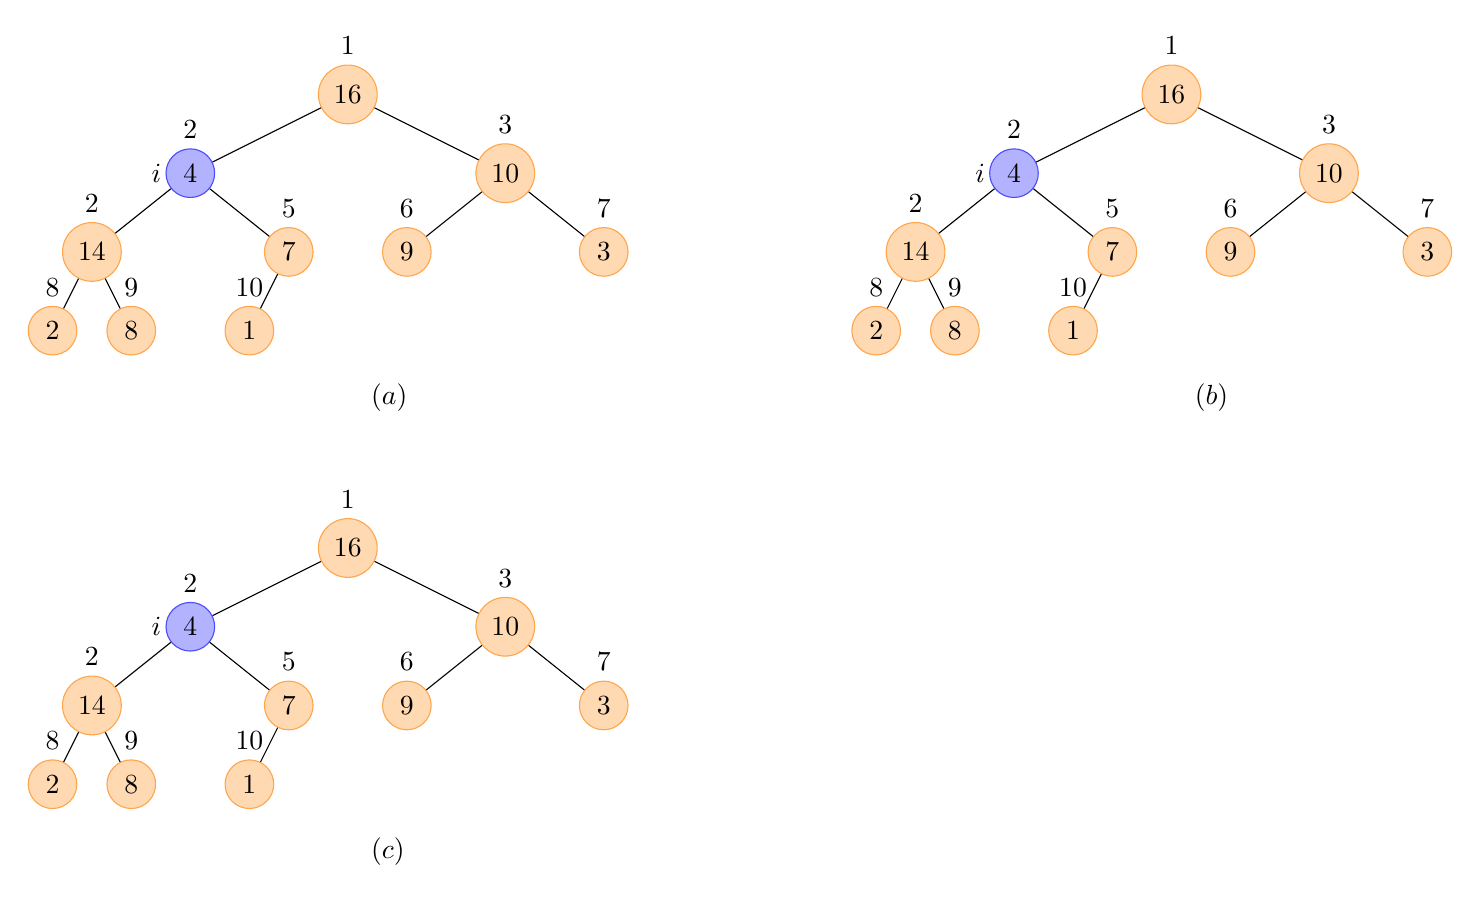
\begin{tikzpicture}[
		level distance = 10mm,				
		level 1/.style = {sibling distance = 40mm},
		level 2/.style = {sibling distance = 25mm},
		level 3/.style = {sibling distance = 10mm}
		]
\node[circle, draw = orange!70, fill = orange!30, label = above:{$1$}] (root1){16}
	child{node[circle, draw = blue!70, fill = blue!30, label = above:{$2$}](4){4}
		child{node[circle, draw = orange!70, fill = orange!30, label = above:{$2$}]{14}
			child{node[circle, draw = orange!70, fill = orange!30, label = above:{$8$}]{2}}
			child{node[circle, draw = orange!70, fill = orange!30, label = above:{$9$}]{8}}			
		}
		child{node[circle, draw = orange!70, fill = orange!30, label = above:{$5$}]{7}
			child{node[circle, draw = orange!70, fill = orange!30, label = above:{$10$}]{1}}
			child[missing]{node{}}	
		}		
	}
	child{node[circle, draw = orange!70, fill = orange!30, label = above:{$3$}]{10}
			child{node[circle, draw = orange!70, fill = orange!30, label = above:{$6$}]{9}}
			child{node[circle, draw = orange!70, fill = orange!30, label = above:{$7$}]{3}}			
		};
		\node[circle, draw = white, fill = white, label = right:{$i$}][left = 3mm of {4}]{};
		\node[circle, draw = white, fill = white, label = right:{$(a)$}][below=3.3cm of {root1}]{};
		
\node[circle, draw = orange!70, fill = orange!30, label = above:{$1$}][right= 97mm of {root1}] (root2){16}
	child{node[circle, draw = blue!70, fill = blue!30, label = above:{$2$}](four){4}
		child{node[circle, draw = orange!70, fill = orange!30, label = above:{$2$}]{14}
			child{node[circle, draw = orange!70, fill = orange!30, label = above:{$8$}]{2}}
			child{node[circle, draw = orange!70, fill = orange!30, label = above:{$9$}]{8}}			
		}
		child{node[circle, draw = orange!70, fill = orange!30, label = above:{$5$}]{7}
			child{node[circle, draw = orange!70, fill = orange!30, label = above:{$10$}]{1}}
			child[missing]{node{}}	
		}		
	}
	child{node[circle, draw = orange!70, fill = orange!30, label = above:{$3$}]{10}
			child{node[circle, draw = orange!70, fill = orange!30, label = above:{$6$}]{9}}
			child{node[circle, draw = orange!70, fill = orange!30, label = above:{$7$}]{3}}			
		};
		\node[circle, draw = white, fill = white, label = right:{$i$}][left = 3mm of {four}]{};
		\node[circle, draw = white, fill = white, label = right:{$(b)$}][below=3.3cm of {root2}]{};
		
		\node[circle, draw = orange!70, fill = orange!30, label = above:{$1$}][below = 50mm of {root1}] (root3){16}
	child{node[circle, draw = blue!70, fill = blue!30, label = above:{$2$}](four){4}
		child{node[circle, draw = orange!70, fill = orange!30, label = above:{$2$}]{14}
			child{node[circle, draw = orange!70, fill = orange!30, label = above:{$8$}]{2}}
			child{node[circle, draw = orange!70, fill = orange!30, label = above:{$9$}]{8}}			
		}
		child{node[circle, draw = orange!70, fill = orange!30, label = above:{$5$}]{7}
			child{node[circle, draw = orange!70, fill = orange!30, label = above:{$10$}]{1}}
			child[missing]{node{}}	
		}		
	}
	child{node[circle, draw = orange!70, fill = orange!30, label = above:{$3$}]{10}
			child{node[circle, draw = orange!70, fill = orange!30, label = above:{$6$}]{9}}
			child{node[circle, draw = orange!70, fill = orange!30, label = above:{$7$}]{3}}			
		};
		\node[circle, draw = white, fill = white, label = right:{$i$}][left = 3mm of {four}]{};
		\node[circle, draw = white, fill = white, label = right:{$(c)$}][below=3.3cm of {root3}]{};

\end{tikzpicture}
\end{center}
\vspace{1cm}

\section{}
\vspace{1cm}
\begin{adjustbox}{width = \textwidth}
%\begin{center}
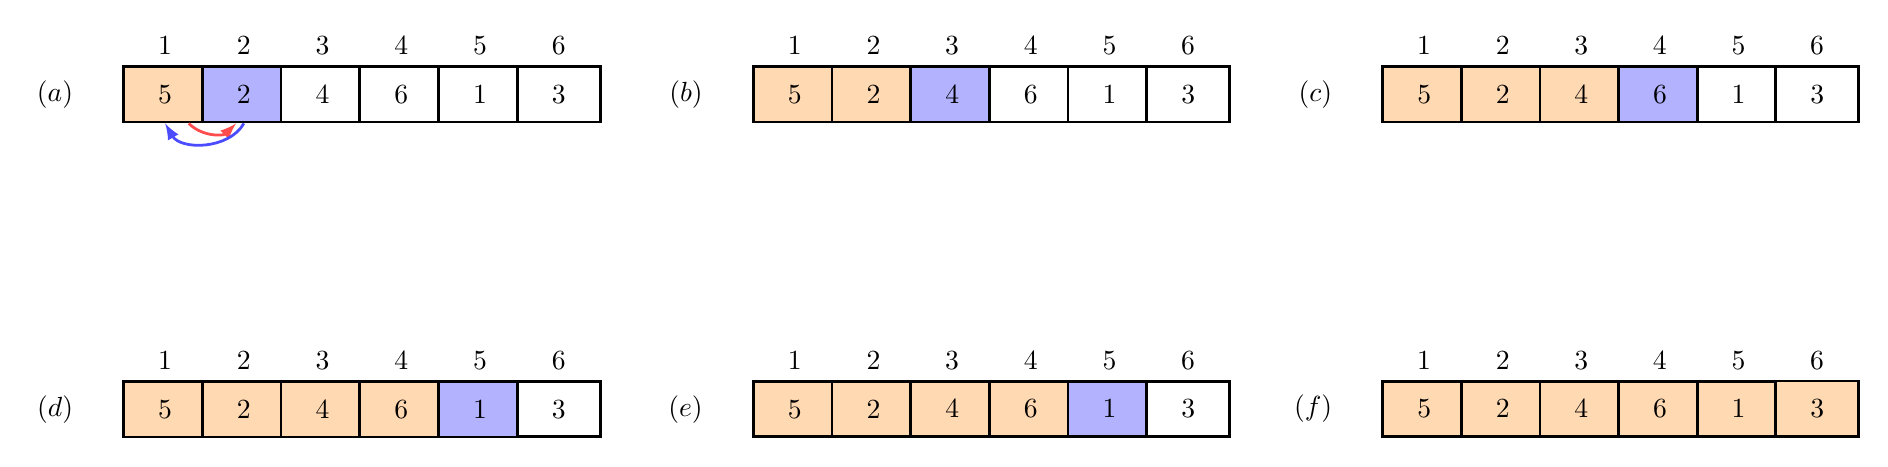
\begin{tikzpicture}[auto,
		alpha_node/.style = {circle, draw = white, inner sep = 0pt},
		blue_node/.style = {rectangle, draw, fill = blue!30!, minimum height = 	2em, minimum width = 3em, inner sep = 0pt},
		orange_node/.style = {rectangle, draw, fill = orange!30!, minimum height = 2em, minimum width = 3em, inner sep = 0pt},
		white_node/.style = {rectangle, draw, fill = white, minimum height = 2em, minimum width = 3em, inner sep = 0pt},
		scale = 5,
		->, 
    		line width=1pt, % Increase the thickness of the arrow lines
    		>=latex, scale=2, % Scale the arrowheads
		]
		
		%a
		\node[alpha_node, label = left:{$(a)$}](a){};
		\node[orange_node, right of = {a}, label = above:{$1$}](1){5};
		\node[blue_node, right of = {1}, label = above:{$2$}](2){2};
		\node[white_node, right of = {2}, label = above:{$3$}](3){4};
		\node[white_node, right of = {3}, label = above:{$4$}](4){6};
		\node[white_node, right of = {4}, label = above:{$5$}](5){1};
		\node[white_node, right of = {5}, label = above:{$6$}](6){3};
		
		\draw[->, bend right = 45, draw = red!70]([xshift = .3mm]1.south) to ([xshift = -.1mm]2.south);
		\path[>=latex, bend left = 60, draw = blue!70](2.south) to (1.south);
		
		%b
		\node[alpha_node, label = left:{$(b)$}][left of = {6}, xshift = 3cm](b){};
		\node[orange_node, right of = {b}, label = above:{$1$}](7){5};
		\node[orange_node, right of = {7}, label = above:{$2$}](8){2};
		\node[blue_node, right of = {8}, label = above:{$3$}](9){4};
		\node[white_node, right of = {9}, label = above:{$4$}](10){6};
		\node[white_node, right of = {10}, label = above:{$5$}](11){1};
		\node[white_node, right of = {11}, label = above:{$6$}](12){3};
		
		%c
		\node[alpha_node, label = left:{$(c)$}][left of = {12}, xshift = 3cm](c){};
		\node[orange_node, right of = {c}, label = above:{$1$}](13){5};
		\node[orange_node, right of = {13}, label = above:{$2$}](14){2};
		\node[orange_node, right of = {14}, label = above:{$3$}](15){4};
		\node[blue_node, right of = {15}, label = above:{$4$}](16){6};
		\node[white_node, right of = {16}, label = above:{$5$}](17){1};
		\node[white_node, right of = {17}, label = above:{$6$}](18){3};
		
		%d
		\node[alpha_node, label = left:{$(d)$}][below of = {a}, yshift = -3cm](d){};
		\node[orange_node, right of = {d}, label = above:{$1$}](19){5};
		\node[orange_node, right of = {19}, label = above:{$2$}](20){2};
		\node[orange_node, right of = {20}, label = above:{$3$}](21){4};
		\node[orange_node, right of = {21}, label = above:{$4$}](22){6};
		\node[blue_node, right of = {22}, label = above:{$5$}](23){1};
		\node[white_node, right of = {23}, label = above:{$6$}](24){3};
		
		%e
		\node[alpha_node, label = left:{$(e)$}][left of = {24}, xshift = 3cm](e){};
		\node[orange_node, right of = {e}, label = above:{$1$}](25){5};
		\node[orange_node, right of = {25}, label = above:{$2$}](26){2};
		\node[orange_node, right of = {26}, label = above:{$3$}](27){4};
		\node[orange_node, right of = {27}, label = above:{$4$}](28){6};
		\node[blue_node, right of = {28}, label = above:{$5$}](29){1};
		\node[white_node, right of = {29}, label = above:{$6$}](30){3};
		
		%f
		\node[alpha_node, label = left:{$(f)$}][left of = {30}, xshift = 3cm](f){};
		\node[orange_node, right of = {f}, label = above:{$1$}](31){5};
		\node[orange_node, right of = {31}, label = above:{$2$}](32){2};
		\node[orange_node, right of = {32}, label = above:{$3$}](33){4};
		\node[orange_node, right of = {33}, label = above:{$4$}](34){6};
		\node[orange_node, right of = {34}, label = above:{$5$}](35){1};
		\node[orange_node, right of = {35}, label = above:{$6$}](36){3};

\end{tikzpicture}
%\end{center}
\end{adjustbox}
\vspace{1cm}

\section{}
\vspace{1cm}
\begin{center}
\begin{tikzpicture}[
	level distance = 1.5cm,
	level 1/.style = {sibling distance = 5cm},
	level 2/.style = {sibling distance = 2.5cm},
	level 3/.style = {sibling distance = 1.25cm},
	every node/.style = {draw = none, anchor = north}
	]
	
	\node (root) {$c_2n$}
		%child {node {$\frac{c_2n}{2}$}
		child {node {${c_2n / 2}$}
			child {node{${c_2n / 4}$}
				child {node (1) {}}
				child {node (2) {}}
				}
			child {node{${c_2n / 4}$}
				child {node (3) {}}
				child {node (4) {}}
				}			
			}
		child {node (lab1) {${c_2n / 2}$}
			child {node{${c_2n / 4}$}
				child {node (5) {}}
				child {node (6) {}}
				}
			child {node (lab2) {${c_2n / 4}$}
				child {node (7) {}}
				child {node (8) {}}
				}			
			};
			
	\node[below of = {1}, yshift = 1.1cm](a){};
	\node[below of = {a}, xshift = -.2cm, yshift = 4.6mm](b){};
	\draw[dashed, thick] (a) -- (b);
	
	\node[below of = {a}, yshift = -.5cm, xshift = -2mm](aa){};
	\node[below of = {aa}, yshift = -.1cm](x){$c_1$};
	\draw[dashed] (aa) -- (x);
	
	\node[below of = {2}, yshift = 1.1cm](i){};
	\node[below of = {i}, xshift = .2cm, yshift = 4.6mm](j){};
	\draw[dashed, thick] (i) -- (j);
	
	\node[below of = {i}, yshift = -.5cm, xshift = -6mm](cc){};
	\node[below of = {cc}, yshift = -.1cm](z){$c_1$};
	\draw[dashed] (cc) -- (z);
	
	
	
	\node[below of = {i}, yshift = -.5cm, xshift = 2mm](bb){};
	\node[below of = {bb}, yshift = -.1cm](y){$c_1$};
	\draw[dashed] (bb) -- (y);
	\node[right of = {bb}, xshift = -.1cm](dd){};
	\node[below of = {dd}, yshift = -.1cm](xx){$c_1$};
	\draw[dashed] (dd) -- (xx);
	\node[right of = {dd}, xshift = -.1cm](ee){};
	\node[below of = {ee}, yshift = -.1cm](yy){$c_1$};
	\draw[dashed] (ee) -- (yy);
	\node[right of = {ee}, xshift = -.1cm](ff){};
	\node[below of = {ff}, yshift = -.1cm](zz){$c_1$};
	\draw[dashed] (ff) -- (zz);
	\node[right of = {ff}, xshift = -.1cm](gg){};
	\node[below of = {gg}, yshift = -.1cm](xxx){$c_1$};
	\draw[dashed] (gg) -- (xxx);
	\node[right of = {gg}, xshift = -.1cm](hh){};
	\node[below of = {hh}, yshift = -.1cm](yyy){$c_1$};
	\draw[dashed] (hh) -- (yyy);
	
	\node[circle, draw = black, fill = black, inner sep = 0.6pt, right of = {yyy}, xshift = -.5cm](dot1){};
	\node[circle, draw = black, fill = black, inner sep = 0.6pt, right of = {dot1}, xshift = -.7cm](dot2){};
	\node[circle, draw = black, fill = black, inner sep = 0.6pt, right of = {dot2}, xshift = -.7cm](dot3){};
	\node[right of = {hh}, xshift = .6cm](ii){};
	\node[below of = {ii}, yshift = -.1cm](zzz){$c_1$};
	\draw[dashed] (ii) -- (zzz);
	\node[right of = {ii}, xshift = -.1cm](jj){};
	\node[below of = {jj}, yshift = -.1cm](kkk){$c_1$};
	\draw[dashed] (kkk) -- (jj);
	\node[right of = {jj}, xshift = -.1cm](kk){};
	\node[below of = {kk}, yshift = -.1cm](kkkk){$c_1$};
	\node[right of = {kkk}, xshift = 1.9cm](lab4){$c_2n$};
	\draw[dashed] (kkkk) -- (kk);
	\draw[->, >=latex, thick, blue] (kkkk)--(lab4);
	
	
	\node[below of = {3}, yshift = 1.1cm](c){};
	\node[below of = {c}, xshift = -.2cm, yshift = 4.6mm](d){};
	\draw[dashed, thick] (c) -- (d);
	
	\node[below of = {4}, yshift = 1.1cm](k){};
	\node[below of = {k}, xshift = .2cm, yshift = 4.6mm](l){};
	\draw[dashed, thick] (k) -- (l);
	
	\node[below of = {5}, yshift = 1.1cm](e){};
	\node[below of = {e}, xshift = -.2cm, yshift = 4.6mm](f){};
	\draw[dashed, thick] (e) -- (f);
	
	\node[below of = {6}, yshift = 1.1cm](m){};
	\node[below of = {m}, xshift = .2cm, yshift = 4.6mm](n){};
	\draw[dashed, thick] (m) -- (n);
	
	\node[below of = {7}, yshift = 1.1cm](g){};
	\node[below of = {g}, xshift = -.2cm, yshift = 4.6mm](h){};
	\draw[dashed, thick] (g) -- (h);
	
	\node[below of = {8}, yshift = 1.1cm](o){};
	\node[below of = {o}, xshift = .2cm, yshift = 4.6mm](p){};
	\draw[dashed, thick] (o) -- (p);
	
	\node[right of = {root}, label = right: {$c_2n$}, xshift = 5cm](c2n1){};
	\draw[->, >=latex, thick, blue] (root)--(c2n1);
	\node[right of = {lab1}, label = right: {$c_2n$}, xshift = 2.6cm](c2n2){};
	\draw[->, >=latex, thick, blue] (lab1)--(c2n2);
	\node[right of = {lab2}, label = right: {$c_2n$}, xshift = 1.5cm](c2n3){};
	\draw[->, >=latex, thick, blue] (lab2)--(c2n3);
	
	
	\node[circle, draw = black, fill = black, inner sep = 0.6pt, below of = {c2n3}, xshift = 5mm, yshift = -6mm](dot4){};
	\node[circle, draw = black, fill = black, inner sep = 0.6pt, below of = {dot4}, yshift = 7mm](dot5){};
	\node[circle, draw = black, fill = black, inner sep = 0.6pt, below of = {dot5}, yshift = 7mm](dot6){};
	
	\node[below of = {lab4}, xshift = -.3cm](start){};
	\node[right of = {start}, xshift = 0cm](end){};
	\draw[thick, black](start)--(end);
	\node[below of = {start}](total){Total: $c_2n \lg n + c_1n$};
	
	\draw[{Latex[length = 3mm]}-{Latex[length = 3mm]}, thick, red](-6, 0) -- ++(0, -8) node[midway, fill = white, text = black] {$\lg n + 1$};
	
	% Drawing a horizontal curly brace that spans 2cm
	\draw [decorate, decoration={brace,amplitude=10pt,mirror,mirror}] (-5, -9) -- (5,-9);
	\node[text = black, xshift = 2mm] at (0, -10){$n$};

\end{tikzpicture}
\end{center}

\end{document}